\section{Result}

\subsection{Hierarchical Clustering}

\subsubsection{Evaluation}

\begin{figure}[H]
    \centering
    \begin{tabular}{|l|c|}
        \hline
        \rowcolor{gray!50}
        & Value \\ \hline
        \textbf{Silhouette Score} & $0.169$ \\ \hline
        \textbf{Dunn Index} & $0.009$ \\ \hline
    \end{tabular}
    \caption{Evaluation metrics for Hierarchical Clustering}\label{fig:Hierarchical_evaluation}
\end{figure}

\subsubsection{Visualization of the clusters:}
\begin{figure}[H]
    \centering
    \begin{subfigure}[b]{0.45\textwidth}
        \centering
        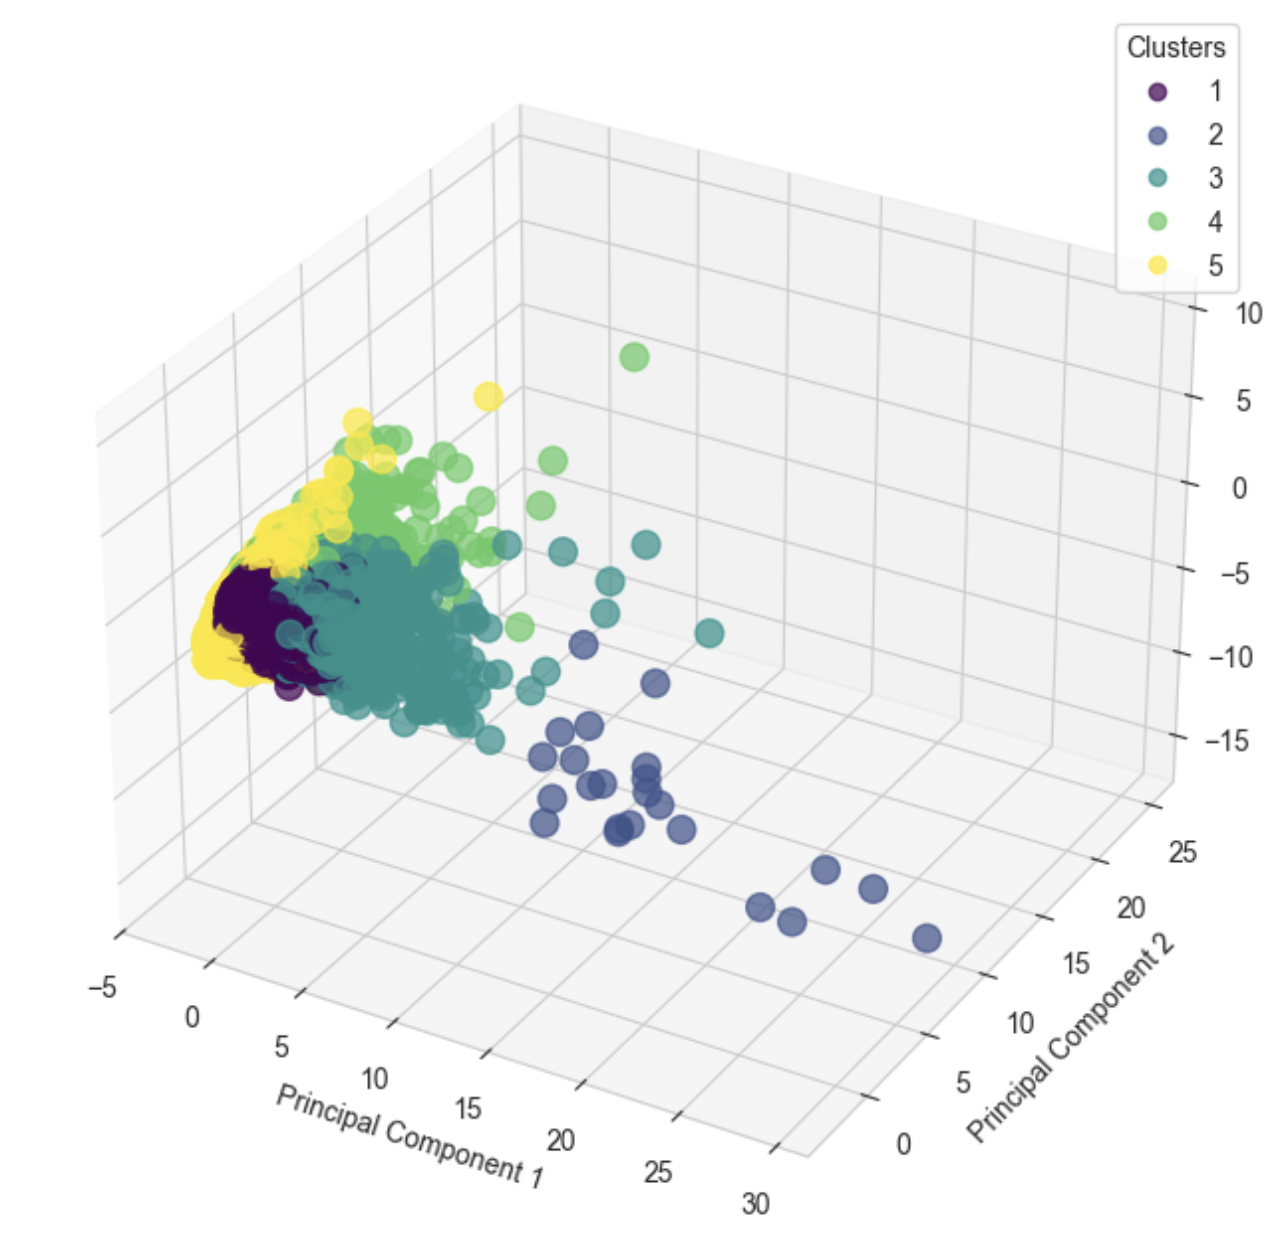
\includegraphics[width=\textwidth]{src/figs/3d_PCA_HC.png}
        \caption{3D PCA visualization of clusters}
        \label{fig:3D_pca}
    \end{subfigure}
    \hfill
    \begin{subfigure}[b]{0.45\textwidth}
        \centering
        \raisebox{0.3cm}{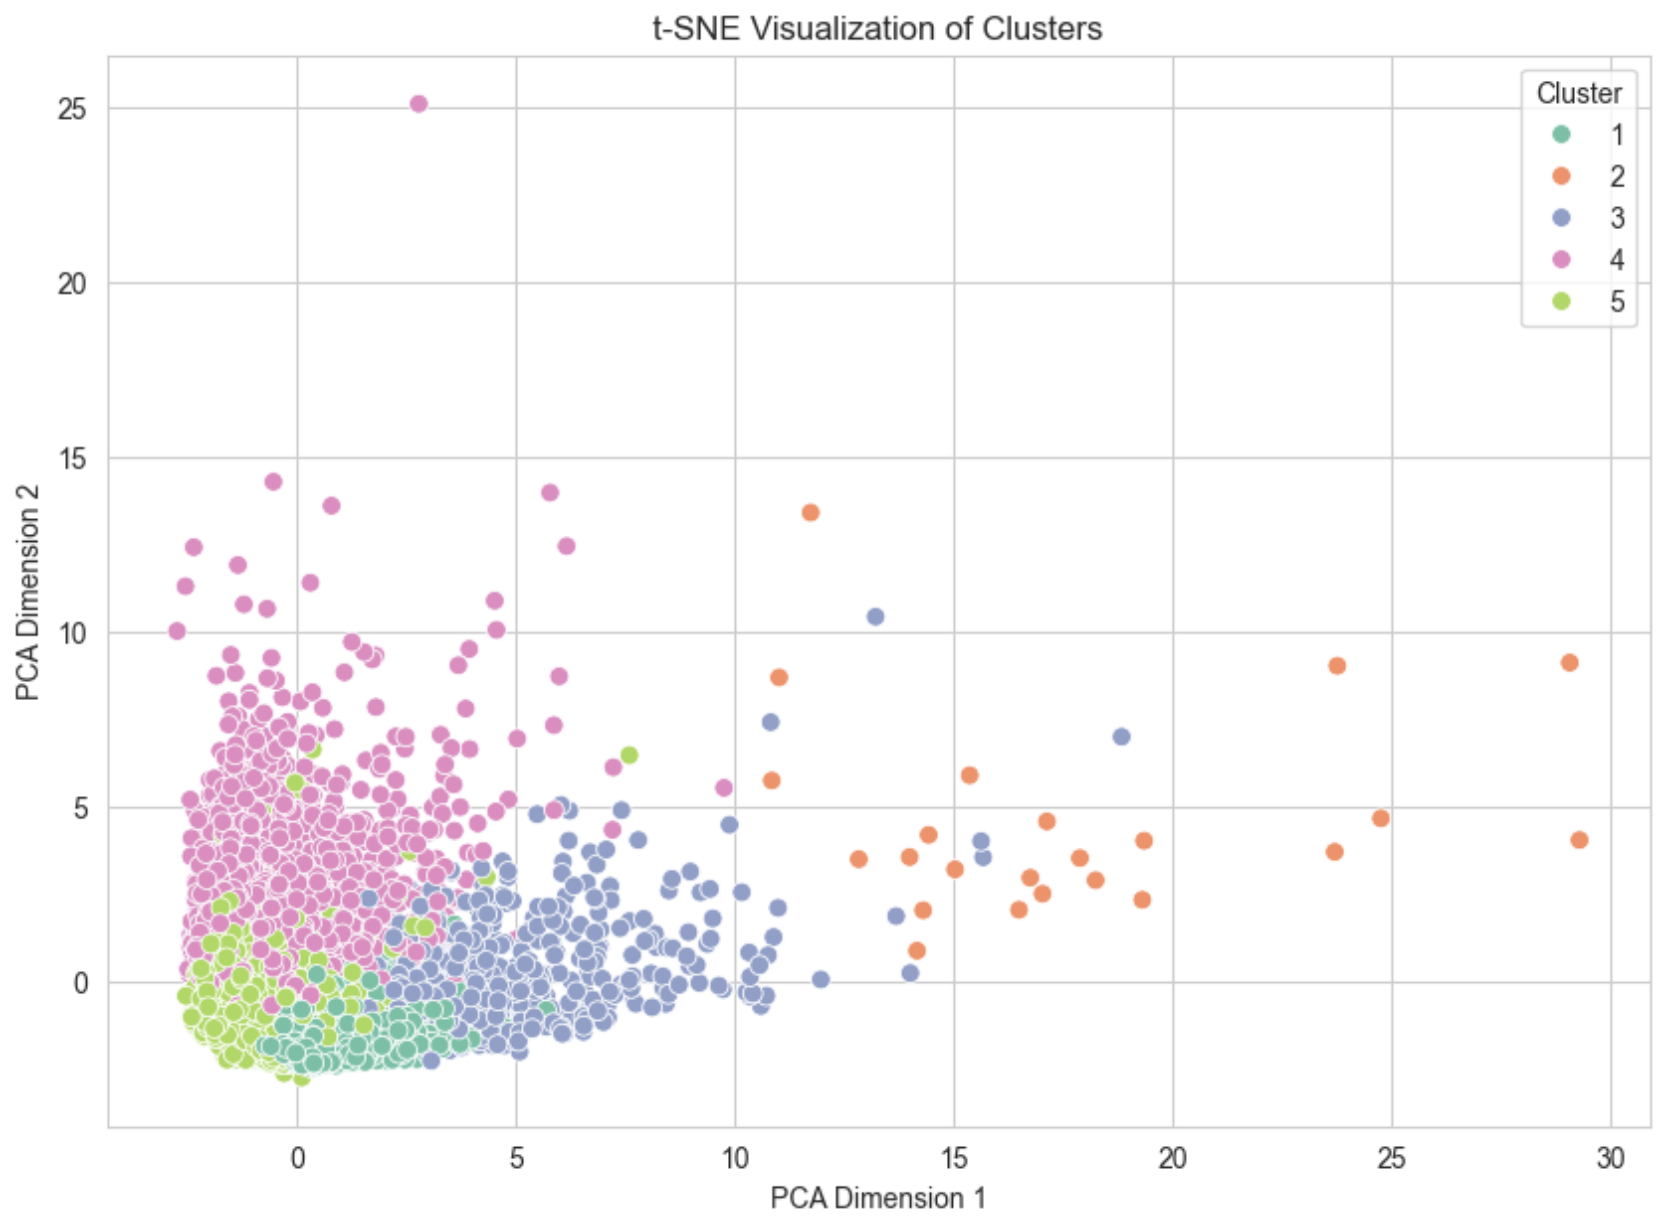
\includegraphics[width=\textwidth]{src/figs/2d_PCA_HC.png}} % Adjusts the image height
        \caption{2D PCA visualization of clusters}
        \label{fig:PCA_2d}
    \end{subfigure}
    \caption{Clustering visualizations: 3D (left) and 2D (right).}
    \label{fig:comparison1}
\end{figure}

\begin{figure}[H]
    \centering
    \begin{subfigure}[b]{0.45\textwidth}
        \centering
        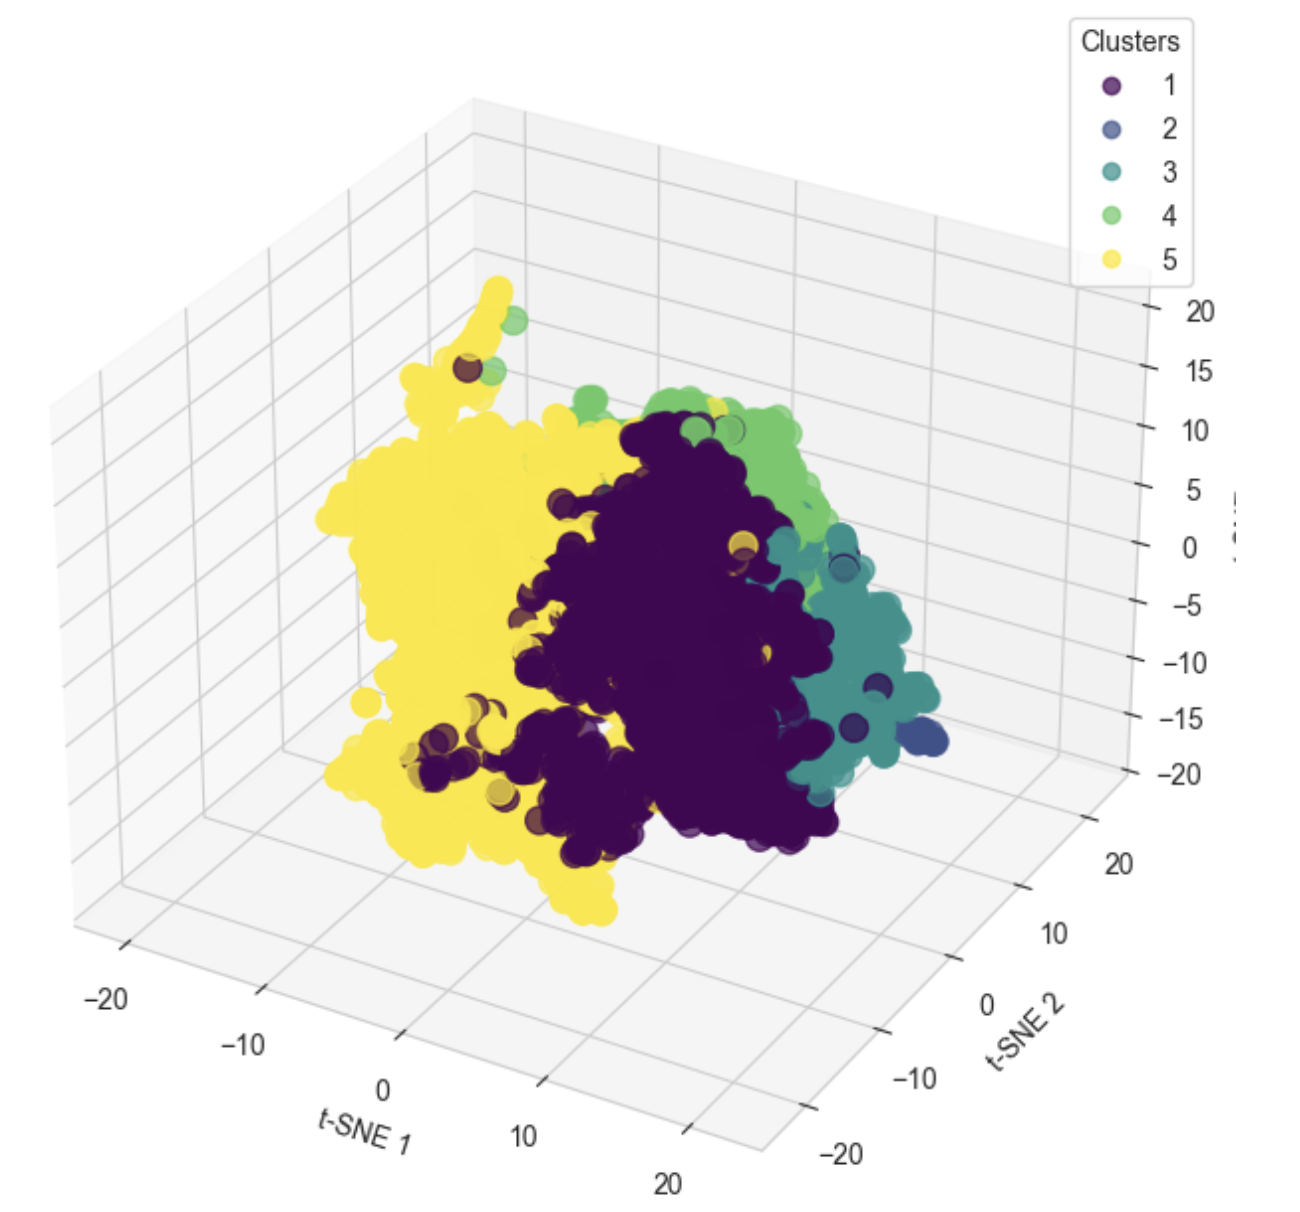
\includegraphics[width=\textwidth]{src/figs/3d_t-SNE.png}
        \caption{3D t-SNE visualization of clusters}
        \label{fig:3D_tsne}
    \end{subfigure}
    \hfill
    \begin{subfigure}[b]{0.45\textwidth}
        \centering
        \raisebox{0.3cm}{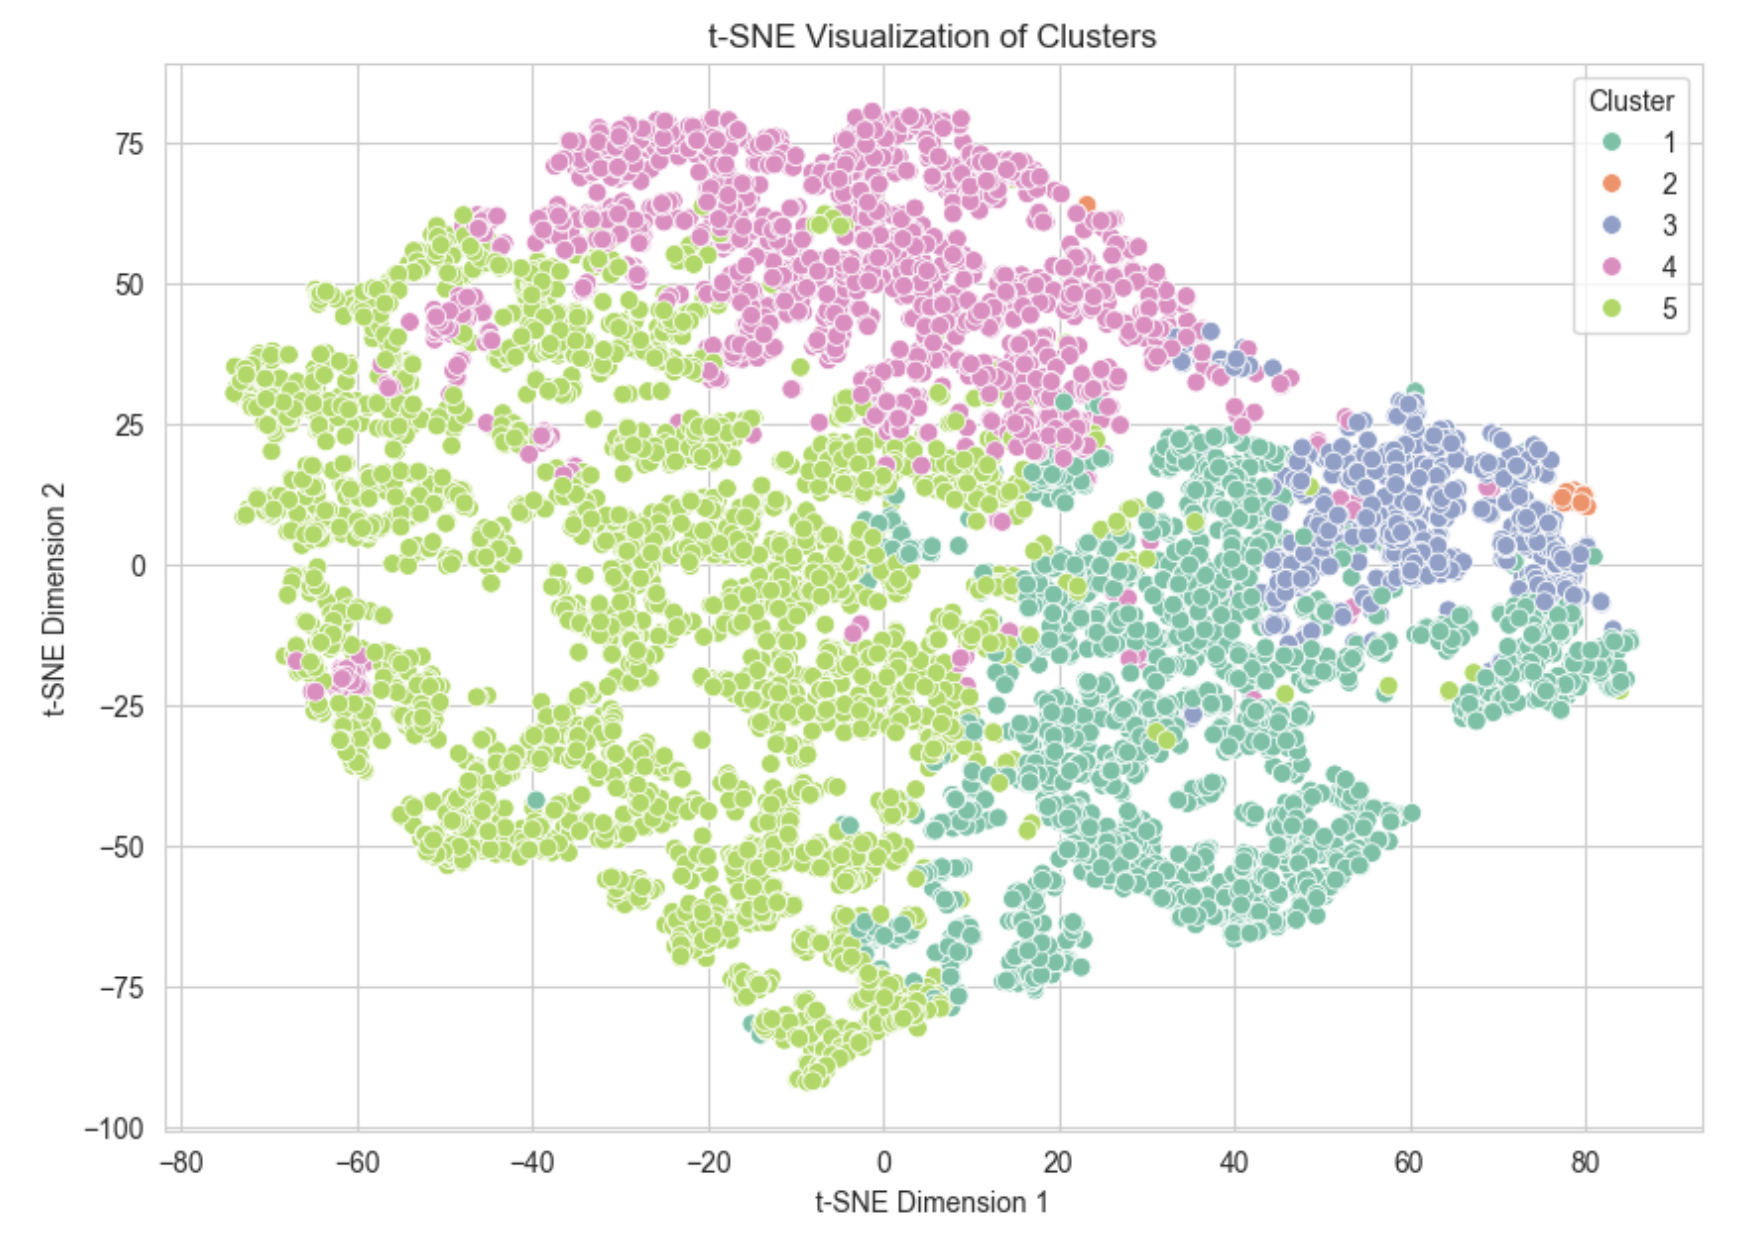
\includegraphics[width=\textwidth]{src/figs/2d_t-SNE.png}} % Adjusts the image height
        \caption{2D t-SNE visualization of clusters}
        \label{fig:2D_tsne}
    \end{subfigure}
    \caption{Clustering visualizations: 3D (left) and 2D (right).}
    \label{fig:comparison2}
\end{figure}

\subsubsection{Cluster Descriptions}
Clarification on what the clusters contain and represent. The clusters are described as follows:
\vspace{0.3cm}
\par
\begin{center}
\textbf{Cluster 1: Medium Activity, Low Spenders with Higher Full Payment Rate}
\begin{table}[H]
\centering
\begin{tabular}{|l|c|c|}
\hline
\textbf{Feature} & \textbf{Values} & \textbf{Interpretation} \\ \hline
Balance & 587.98 & Low \\ \hline
Purchases & 1203.26 & Low \\ \hline
One-Off Purchases & 542.97 & Moderate \\ \hline
Installments Purchases & 660.38 & Moderate \\ \hline
Cash Advance & 69.96 & Low \\ \hline
Credit Limit & 4157.06 & Moderate \\ \hline
Payments & 1269.62 & Moderate \\ \hline
Full Payment Percentage & 0.35 & Moderate \\ \hline
Cluster size & 2228.00 & Moderate \\ \hline
\end{tabular}
\caption{Cluster 1 description.}
\end{table}

\centering
\textbf{Cluster 2: High Spenders with Large Balances and High Full Payment Rate}
\begin{table}[H]
\centering
\begin{tabular}{|l|c|c|}
\hline
\textbf{Feature} & \textbf{Values} & \textbf{Interpretation} \\ \hline
Balance & 4812.38 & Very High \\ \hline
Purchases & 27505.34 & Very High \\ \hline
One-Off Purchases & 22417.45 & Very High \\ \hline
Installments Purchases & 5087.89 & Very High \\ \hline
Cash Advance & 1617.79 & High \\ \hline
Credit Limit & 16000.00 & Very High \\ \hline
Payments & 28138.98 & Very High \\ \hline
Full Payment Percentage & 0.53 & High \\ \hline
Cluster size & 23.00 & Very Low \\ \hline
\end{tabular}
\caption{Cluster 2 description.}
\end{table}

\centering
\textbf{Cluster 3: Moderate Credit Usage with Low Full Payment Rate}
\begin{table}[H]
\centering
\begin{tabular}{|l|c|c|}
\hline
\textbf{Feature} & \textbf{Values} & \textbf{Interpretation} \\ \hline
Balance & 3093.29 & High \\ \hline
Purchases & 5059.38 & Moderate \\ \hline
One-Off Purchases & 3176.73 & Moderate \\ \hline
Installments Purchases & 1883.64 & Moderate \\ \hline
Cash Advance & 427.99 & Moderate \\ \hline
Credit Limit & 8084.07 & High \\ \hline
Payments & 4411.09 & Moderate \\ \hline
Full Payment Percentage & 0.18 & Low \\ \hline
Cluster size & 609.00 & Low \\ \hline
\end{tabular}
\caption{Cluster 3 description.}
\end{table}

\centering
\textbf{Cluster 4: Customers with Low Purchases, High Cash Advances, and Low Full Payment}
\begin{table}[H]
\centering
\begin{tabular}{|l|c|c|}
\hline
\textbf{Feature} & \textbf{Values} & \textbf{Interpretation} \\ \hline
Balance & 3753.04 & High \\ \hline
Purchases & 536.14 & Low \\ \hline
One-Off Purchases & 311.82 & Low \\ \hline
Installments Purchases & 224.39 & Low \\ \hline
Cash Advance & 3412.73 & Very High \\ \hline
Credit Limit & 6304.57 & High \\ \hline
Payments & 2908.71 & Low \\ \hline
Full Payment Percentage & 0.04 & Low \\ \hline
Cluster size & 1796.00 & Moderate \\ \hline
\end{tabular}
\caption{Cluster 4 description.}
\end{table}

\centering
\textbf{Cluster 5: Low Usage of Credit with Minimal Purchases or Payments}
\begin{table}[H]
\centering
\begin{tabular}{|l|c|c|}
\hline
\textbf{Feature} & \textbf{Values} & \textbf{Interpretation} \\ \hline
Balance & 950.55 & Low \\ \hline
Purchases & 376.41 & Low \\ \hline
One-Off Purchases & 252.25 & Low \\ \hline
Installments Purchases & 124.60 & Low \\ \hline
Cash Advance & 503.19 & Low \\ \hline
Credit Limit & 3310.72 & Low \\ \hline
Payments & 1011.16 & Low \\ \hline
Full Payment Percentage & 0.10 & Low \\ \hline
Cluster size & 3980.00 & High \\ \hline
\end{tabular}
\caption{Cluster 5 description.}
\end{table}
\end{center}

\subsection{DBSCAN}

\subsubsection{Evaluation}

\begin{figure}[H]
    \centering
    \begin{tabular}{|l|c|}
        \hline
        \rowcolor{gray!50}
        & Value \\ \hline
        \textbf{Silhouette Score} & $-0.328$ \\ \hline
        \textbf{Dunn Index} & $0.001$ \\ \hline
    \end{tabular}
    \caption{Evaluation metrics for DBSCAN}\label{fig:DBSCAN_evaluation}
\end{figure}

\subsubsection{Visualization of the clusters:}

The clusters we get from DBSCAN are visualized in 3D using PCA and t-SNE. First we visualize the clusters including the $-1$ cluster, which represents the outliers. Then we visualize the clusters without the $-1$ cluster, to get a better view of the clusters that DBSCAN finds.

\begin{figure}[H]
    \hspace*{\fill}
    \centering
    \begin{subfigure}[b]{0.45\textwidth}
        \centering
        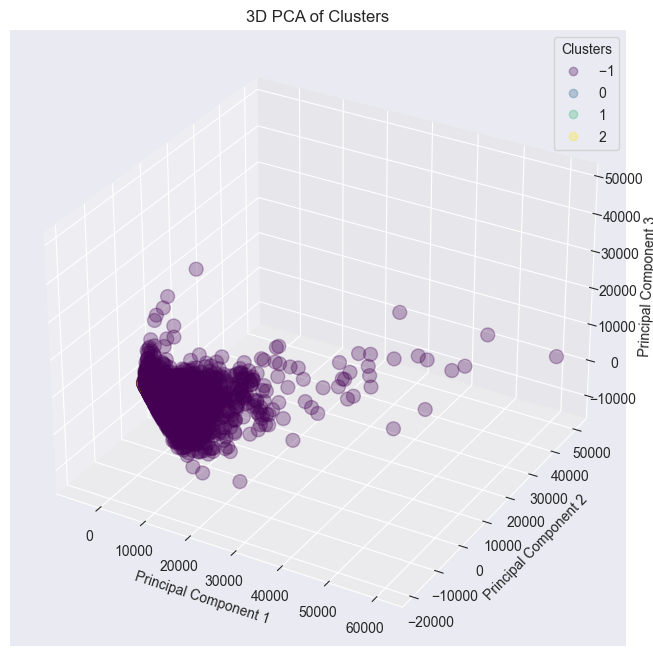
\includegraphics[width=1.0\textwidth]{src/figs/3d_PCA_DBSCAN_with.png} 
        \caption{3D PCA with $-1$ cluster}\label{fig:DBSCAN_PCA_with}
    \end{subfigure}
    \hfill
    \begin{subfigure}[b]{0.45\textwidth}
        \centering
        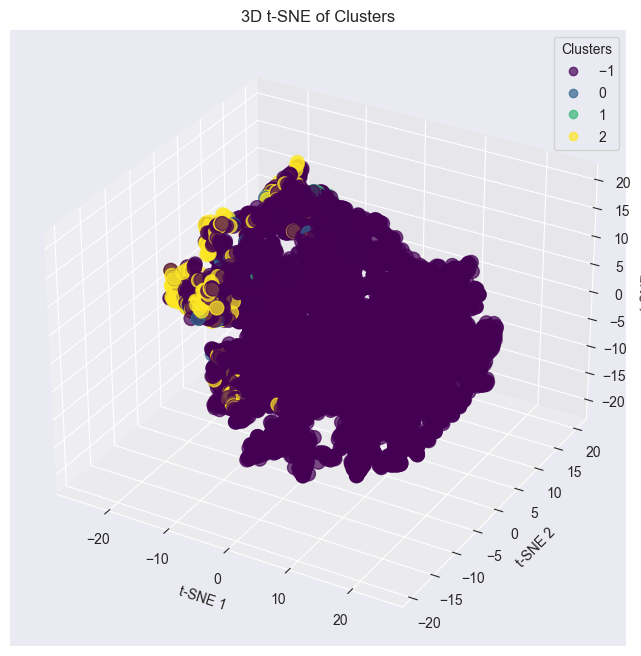
\includegraphics[width=1.0\textwidth]{src/figs/3d_t-SNE_DBSCAN_with.png} 
        \caption{3D t-SNE with $-1$ cluster}\label{fig:DBSCAN_tsne_with}
    \end{subfigure}
    \caption{Visualization of DBSCAN clusters with $-1$ cluster data included}\label{fig:with_outliers}
    \hspace*{\fill}
\end{figure}

\begin{figure}[H]
    \hspace*{\fill}
    \centering
    \begin{subfigure}[b]{0.45\textwidth}
        \centering
        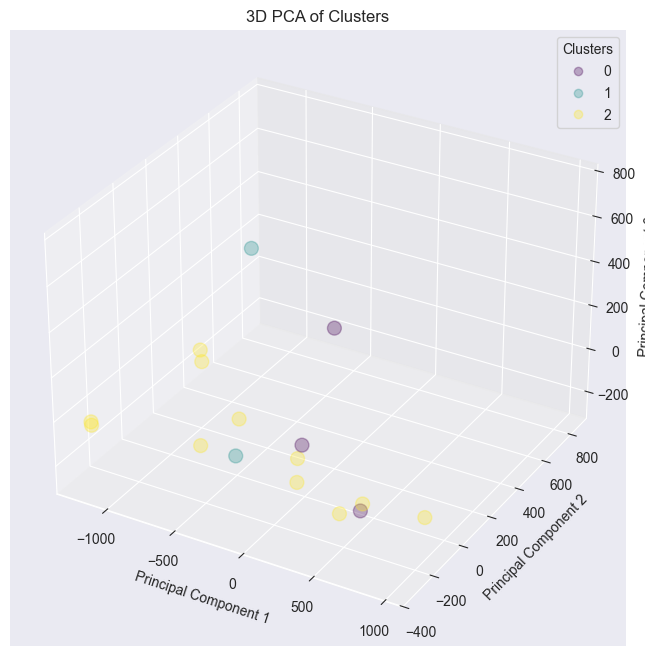
\includegraphics[width=1.0\textwidth]{src/figs/3d_PCA_DBSCAN_without.png} 
        \caption{3D PCA without $-1$ cluster}\label{fig:DBSCAN_PCA_without}
    \end{subfigure}
    \hfill
    \begin{subfigure}[b]{0.45\textwidth}
        \centering
        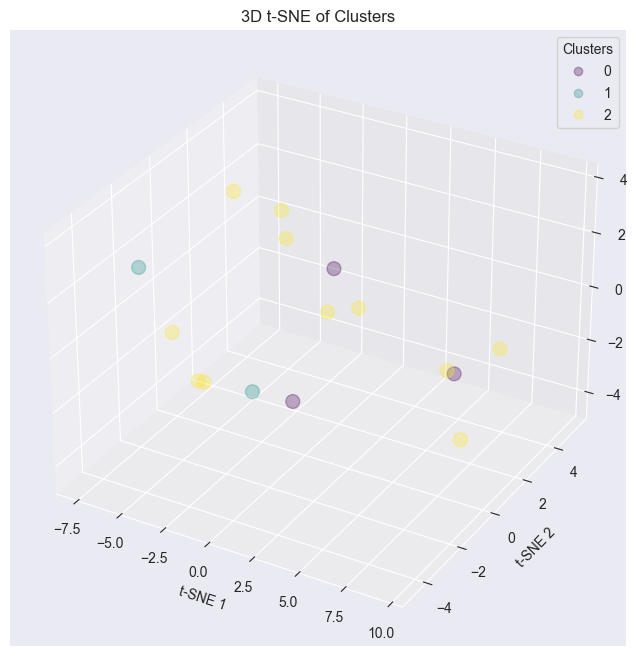
\includegraphics[width=1.0\textwidth]{src/figs/3d_t-SNE_DBSCAN_without.png} 
        \caption{3D t-SNE without $-1$ cluster}\label{fig:DBSCAN_tsne_without}
    \end{subfigure}
    \caption{Visualization of DBSCAN clusters with $-1$ cluster data excluded}\label{fig:without_outliers}
    \hspace*{\fill}
\end{figure}